\solutionSection

\subsubsection*{Спутник}

\begin{enumerate}
    \item Калибровка магнитометра
    \item 
    Используя программу Magneto, необходимо определить калибровочные коэффициенты для магнитометра. После их определения необходимо будет задать функцию калибровки магнитометра:
    
    \inputminted[fontsize=\footnotesize, linenos]{python}{final/command_tour/dzz/task_02/source_1.py}

    Далее для корректного вычисления угла необходимо добавить небольшой пересчёт угла:

    \inputminted[fontsize=\footnotesize, linenos]{python}{final/command_tour/dzz/task_02/source_2.py}

    \item Код ориентации:
    
    \inputminted[fontsize=\footnotesize, linenos]{python}{final/command_tour/dzz/task_02/source_3.py}

\end{enumerate}

\subsubsection*{Оптика}

После сборки оптическая система выглядит следующим образом:

\putTwoImg{7cm}{3}{7cm}{4}

После первичной юстировки можно получить достаточно чёткие изображения с камеры, что невозможно изначально, так как у камеры отсутствует линза и автофокус.

\begin{table}[H]
    \center
    \begin{tabular}{|p{7.5cm}|p{7.5cm}|}
        \hline
        Оригинальная картинка, выставленная на экране смартфона:&
        Картинка с камеры, полученная на расстоянии 4 метра: \\
        \hline
        \hspace{0.5cm}
\includegraphics[width=6cm]{5}
        & 
        \vspace{-8cm}
        \hspace{0.5cm}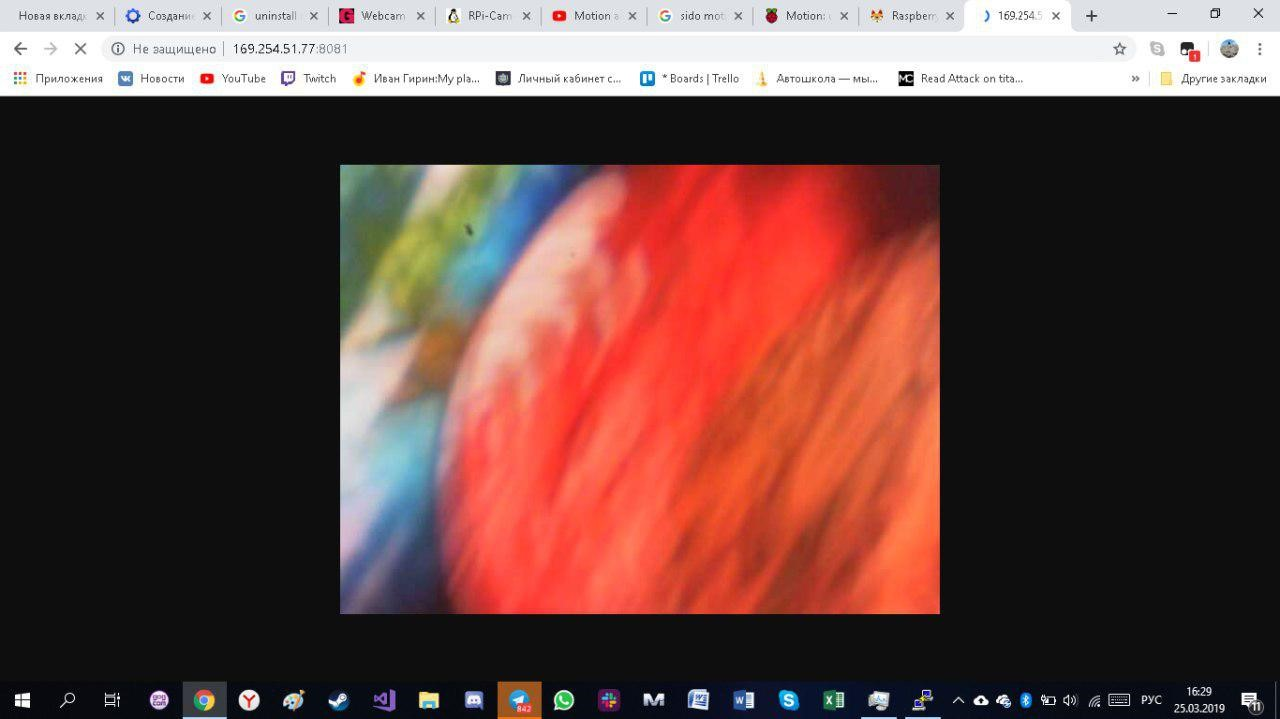
\includegraphics[width=7cm]{6} \\
        \hline
    \end{tabular}
\end{table}

\subsection*{СУПН}

Используя пакет motion можно получить изображение с камеры. Для удобства настройки оптической системы для начала наладим потоковое видео с камеры.

\begin{enumerate}
    \item Подключаемся к Raspberry
    \item Заходим в файл с конфигурациями motion:
    \putImgWOCaption{13cm}{7}
    Далее настраиваем вывод потокового видео, задавая следующие настройки:
    
    start\_motion\_daemon = yes\\
    \dots\\
    stream\_localhost off\\
    \dots\\
    webcontrol\_localhost off
    \item Далее, закрыв файл, включаем трансляцию:
    \putImgWOCaption{13cm}{8}
    Если всё успешно, то в вашем браузере по адресу \url{http://10.42.0.90:8081/} (где 10.42.0.90 - это IP самой Raspberry) начнётся трансляция видео.
    \putImgWOCaption{13cm}{9}
    Так как камера не имеет автофокуса и линзы, изображение будет расфокусированным.
    \item  Ваши фото сохраняются по адресу, заданному в файле motion.conf строкой target\_dir. По умолчанию это home/pi/motion. Вы можете изменить директорию на более удобную. Задав параметры motion.conf можно сделать так, что снимок будет делаться по команде:
    \putImgWOCaption{13cm}{10}
    И сохраняться в указанную вами директорию.
    \item Перед отладкой автоматизированной передачи получаемого камерой снимка на ваш ПК рекомендуется наладить беспроводное соединение между вашим ПК и Raspberry. Самый простой способ - открыв файл wpa\_supplicant.conf и прописав там логин и пароль от сети, в которой находится ваш ПК.
    \item Самый простой способ передать файл - использовать команду scp. 
    \item[6.1.] Необходимо открыть для передачи ssh-порт на вашем ПК. Можно использовать uwf.
    \item[6.2.] После открытия порта будет работать команд scp:
    \putImgWOCaption{13cm}{10} 
    По указанной директории вы увидите свой файл.
    \item Теперь необходимо автоматизировать процесс. Можно написать небольшой python-скрипт, который будет осуществлять указанные действия самостоятельно.
\end{enumerate}

\subsubsection*{Проектирование группировки}

Оптимального решения можно достичь, используя два спутника. Для спутника, размещаемого на орбите, можно выбрать один из трёх типов камеры:

\begin{table}[H]
    \center
    \begin{tabular}{|p{2cm}|p{1.5cm}|p{3.5cm}|p{3.5cm}|p{3.5cm}|}
        \hline
        Тип и диапазон	&Диапазон съемки	&Ширина полосы при размещении на высоте 500 км, в км	&Пространственное разрешение на высоте 500 км, в м	&Условная стоимость аппарата с камерой этого типа  \\
        \hline
        LR1 / ИК	&МС/ИК	&1 250	&600	&5 \\
        \hline
        LR2 / ИК	&МС/ИК	&313	&150	&5 \\
        \hline
        LR3 / ИК	&МС/ИК	&156	&75	&7.5 \\
        \hline
    \end{tabular}
\end{table}

Задача заключается прежде всего в том, чтобы подобрать орбиту таким образом, чтобы она покрыла максимум зоны с допустимым разрешением. Разрешение, в свою очередь ограничивает высоту орбиты.

\textit{Пример решения:}

Известно, что необходимо заснять зону, ограниченную 68$^\circ$ и 78$^\circ$ северной широты, 32$^\circ$ и 74$^\circ$ восточной долготы. Отсюда делаем вывод, что наклонение орбиты не должно быть меньше 78$^\circ$.

Очевидно, что чем больше высота, тем хуже разрешение, но тем больше ширина полосы. 

Рассмотрим случай, когда один спутник находится на низкой орбите. Чем меньше высота орбиты, тем чаще спутник будет делать обороты вокруг Земли. При низких орбитах стоит рассматривать камеру LR1, которая позволит снимать с приемлемым разрешением и достаточно большой шириной захвата.

\putImgWOCaption{15cm}{11}

\putImgWOCaption{15cm}{12}

При подобного рода орбитах получаем проход над интересующей нас зоной:

\putImgWOCaption{7cm}{13}

\putImgWOCaption{14cm}{14}

\subsubsection*{Интеграция}

Самым простым способом является использование стандартной библиотеки спутника, использующейся для работы с подключаемой к его сети Arduino:

$arduino\_send(0, 1, None, 100)$\\
0 - номер Arduino;\\
1 - идентификатор сообщения;\\
None - передаваемые данные;\\
100 - ожидание ответа в мс.

Схема взаимодействия строится следующим образом:

\begin{enumerate}
    \item В БКУ на исполнение запускается программа, содержащая код:
    \inputminted[fontsize=\footnotesize, linenos]{python}{final/command_tour/dzz/task_02/source_5.py}
    \item На ардуино скетч ждёт команду от БКУ и выводит данные в Serial:
    \inputminted[fontsize=\footnotesize, linenos]{cpp}{final/command_tour/dzz/task_02/source_6.cpp}
    \item На Raspberry пишем python-скрипт, который читает Serial:
    \inputminted[fontsize=\footnotesize, linenos]{python}{final/command_tour/dzz/task_02/source_7.py}
\end{enumerate}

В итоге в терминале после запуска созданного вами файла с расширением .py, содержащего код, представленный выше, будет выводиться цифровое значение.